\section{Introduction}

Throughout this chapter, we aim to provide a comprehensive understanding of the methodology employed in our research, laying the foundation for the presentation and discussion of the results in the following chapters.

\section{Artificial Neural Networks (ANNs)}
Artificial Neural Networks (ANNs) are computational models inspired by biological neural systems. They use interconnected layers of artificial neurons to process information and perform tasks like pattern recognition, classification, and regression. ANNs adjust the connections, or "weights," between neurons during learning to improve performance. The concept of neural networks emerged in the mid-20th century with the work of Warren McCulloch and Walter Pitts. Still, modern neural networks began with Frank Rosenblatt's perceptron in 1957, a single-layer network able to learn linearly separable patterns.

%Single neuron
\begin{SCfigure}[2\sidecaptionrelwidth][h]
	\centering
	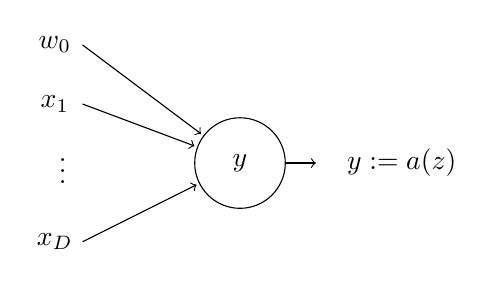
\begin{tikzpicture}[shorten >=1pt,->]
		\tikzstyle{unit}=[draw,shape=circle,minimum size=1.15cm]
 
		\node[unit](p) at (2,1){$y$};
		\node(dots) at (-0.25,1){\vdots};
 
		\draw (0,2.5) node[xshift=-10]{$w_0$} -- (p);
		\draw (0,1.75) node[xshift=-10]{$x_1$} --(p);
		\draw (0,0) node[xshift=-10]{$x_D$} -- (p);
		\draw (p) -- (3,1) node[xshift=30]{$y := a(z)$};
	\end{tikzpicture}
	\caption[Single processing units and its components.]{\small{Single processing unit and its components. The activation function is denoted by $a$ and applied to the actual input $z$ of the unit to form its output $y = a(z)$. $x_1, \ldots, x_D$ represent input from other units within the network; $w_0$ is called bias and represents an external input to the unit. The propagation rule maps all inputs onto the actual input $z$.}}
	\label{fig:processing-unit}
\end{SCfigure}

%NN
\begin{SCfigure}[12][ht]
	\centering
    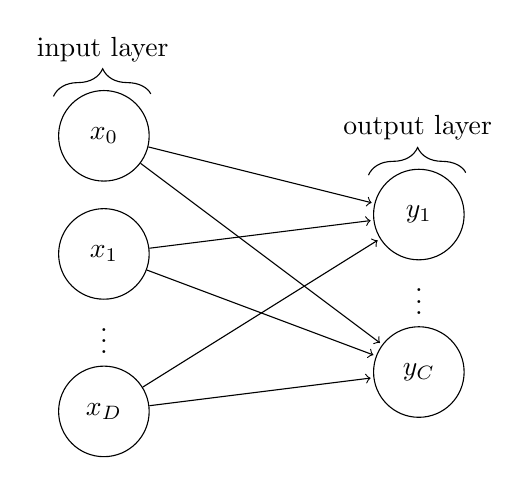
\begin{tikzpicture}[shorten >=1pt]
        \tikzstyle{unit}=[draw,shape=circle,minimum size=1.15cm]
 
        \node[unit](x0) at (0,3.5){$x_0$};
        \node[unit](x1) at (0,2){$x_1$};
        \node(dots) at (0,1){\vdots};
        \node[unit](xd) at (0,0){$x_D$};
 
        \node[unit](y1) at (4,2.5){$y_1$};
        \node(dots) at (4,1.5){\vdots};
        \node[unit](yc) at (4,0.5){$y_C$};
 
        \draw[->] (x0) -- (y1);
        \draw[->] (x0) -- (yc);
 
        \draw[->] (x1) -- (y1);
        \draw[->] (x1) -- (yc);
 
        \draw[->] (xd) -- (y1);
        \draw[->] (xd) -- (yc);
 
        \draw [decorate,decoration={brace,amplitude=10pt},xshift=-4pt,yshift=0pt] (-0.5,4) -- (0.75,4) node [black,midway,yshift=+0.6cm]{input layer};
        \draw [decorate,decoration={brace,amplitude=10pt},xshift=-4pt,yshift=0pt] (3.5,3) -- (4.75,3) node [black,midway,yshift=+0.6cm]{output layer};
    \end{tikzpicture}
    \caption[Network graph of a perceptron with $D$ input units and $C$ output units.]{The perceptron consists of $D$ input units and $C$ output units. All units are labeled according to their output: $y_i = f(z_i)$ in the case of output units; $x_i$ in the case of input units. The input values $x_i$ are propagated to each output unit using the weighted sum propagation rule. The additional input value $x_0 := 1$ is used to include the biases as weights.}
    \label{fig:perceptron}
\end{SCfigure}

It consists of an input layer, one or more hidden layers, and an output layer. Each neuron in a layer receives input from the previous layer and computes an output value using an activation function. The output of the last layer represents the prediction or classification result.

%Activation equation
\begin{figure}
    \centering
    \scalebox{0.8}{
% NEURAL NETWORK activation
% https://www.youtube.com/watch?v=aircAruvnKk&list=PLZHQObOWTQDNU6R1_67000Dx_ZCJB-3pi&index=1
\begin{tikzpicture}[x=2.7cm,y=1.6cm]
\centering
  \message{^^JNeural network activation}
  \def\NI{5} % number of nodes in input layers
  \def\NO{4} % number of nodes in output layers
  \def\yshift{0.4} % shift last node for dots
  
  % INPUT LAYER
  \foreach \i [evaluate={\c=int(\i==\NI); \y=\NI/2-\i-\c*\yshift; \index=(\i<\NI?int(\i):"n");}]
              in {1,...,\NI}{ % loop over nodes
    \node[node in,outer sep=0.6] (NI-\i) at (0,\y) {$a_{\index}^{(0)}$};
  }
  
  % OUTPUT LAYER
  \foreach \i [evaluate={\c=int(\i==\NO); \y=\NO/2-\i-\c*\yshift; \index=(\i<\NO?int(\i):"m");}]
    in {\NO,...,1}{ % loop over nodes
    \ifnum\i=1 % high-lighted node
      \node[node hidden]
        (NO-\i) at (1,\y) {$a_{\index}^{(1)}$};
      \foreach \j [evaluate={\index=(\j<\NI?int(\j):"n");}] in {1,...,\NI}{ % loop over nodes in previous layer
        \draw[connect,white,line width=1.2] (NI-\j) -- (NO-\i);
        \draw[connect] (NI-\j) -- (NO-\i)
          node[pos=0.50] {\contour{white}{$w_{1,\index}$}};
      }
    \else % other light-colored nodes
      \node[node,blue!20!black!80,draw=myblue!20,fill=myblue!5]
        (NO-\i) at (1,\y) {$a_{\index}^{(1)}$};
      \foreach \j in {1,...,\NI}{ % loop over nodes in previous layer
        %\draw[connect,white,line width=1.2] (NI-\j) -- (NO-\i);
        \draw[connect,myblue!20] (NI-\j) -- (NO-\i);
      }
    \fi
  }
  
  % DOTS
  \path (NI-\NI) --++ (0,1+\yshift) node[midway,scale=1.2] {$\vdots$};
  \path (NO-\NO) --++ (0,1+\yshift) node[midway,scale=1.2] {$\vdots$};
  
  % EQUATIONS
  \def\agr#1{{\color{mydarkgreen}a_{#1}^{(0)}}}
  \node[below=17,right=11,mydarkblue,scale=0.95] at (NO-1)
    {$\begin{aligned} %\underset{\text{bias}}{b_1}
       &= \color{mydarkred}\sigma\left( \color{black}
            w_{1,0}\agr{0} + w_{1,1}\agr{1} + \ldots + w_{1,n}\agr{n} + b_1^{(0)}
          \color{mydarkred}\right)\\
       &= \color{mydarkred}\sigma\left( \color{black}
            \sum_{i=1}^{n} w_{1,i}\agr{i} + b_1^{(0)}
           \color{mydarkred}\right)
     \end{aligned}$};
  \node[right,scale=0.9] at (1.3,-1.3)
    {$\begin{aligned}
      {\color{mydarkblue}
      \begin{pmatrix}
        a_{1}^{(1)} \\[0.3em]
        a_{2}^{(1)} \\
        \vdots \\
        a_{m}^{(1)}
      \end{pmatrix}}
      &=
      \color{mydarkred}\sigma\left[ \color{black}
      \begin{pmatrix}
        w_{1,0} & w_{1,1} & \ldots & w_{1,n} \\
        w_{2,0} & w_{2,1} & \ldots & w_{2,n} \\
        \vdots  & \vdots  & \ddots & \vdots  \\
        w_{m,0} & w_{m,1} & \ldots & w_{m,n}
      \end{pmatrix}
      {\color{mydarkgreen}
      \begin{pmatrix}
        a_{1}^{(0)} \\[0.3em]
        a_{2}^{(0)} \\
        \vdots \\
        a_{n}^{(0)}
      \end{pmatrix}}
      +
      \begin{pmatrix}
        b_{1}^{(0)} \\[0.3em]
        b_{2}^{(0)} \\
        \vdots \\
        b_{m}^{(0)}
      \end{pmatrix}
      \color{mydarkred}\right]\\[0.5em]
      {\color{mydarkblue}a^{(1)}}
      &= \color{mydarkred}\sigma\left( \color{black}
           \mathbf{W}^{(0)} {\color{mydarkgreen}a^{(0)}}+\mathbf{b}^{(0)}
         \color{mydarkred}\right)
         %\color{black},\quad \mathbf{W}^{(0)} \in \mathbb{R}^{m\times n}
    \end{aligned}$};

\end{tikzpicture}
}
\caption[Activation function \cite{tikz}.]{\small{The input layer with \textit{n} nodes is denoted as $a_i^{(0)}$ for $i \in \{1, \ldots, n\}$. The output layer with \textit{m} nodes is $a_j^{(1)}$ for $j \in \{1, \ldots, m\}$. Connections between these layers are governed by the weight matrix $\mathbf{W}^{(0)} \in \mathbb{R}^{m\times n}$ and bias vector $\mathbf{b}^{(0)} \in \mathbb{R}^{m}$, with elements $w_{j,i}$ and $b_j^{(0)}$ respectively. The activation function $\sigma$ operates element-wise on the sum of the product of the weight matrix, input vector, and bias vector.}}


    \label{fig:activation_function}

\end{figure}

%Multi-layer_NN
\begin{figure}[ht]
	\centering
	% NEURAL NETWORK with coefficients, shifted
\begin{tikzpicture}[x=2.0cm,y=1.2cm]
  \message{^^JNeural network, shifted}
  \readlist\Nnod{4,5,5,5,3} % array of number of nodes per layer
  \readlist\Nstr{n,m,m,m,k} % array of string number of nodes per layer
  \readlist\Cstr{\strut x,a^{(\prev)},a^{(\prev)},a^{(\prev)},y} % array of coefficient symbol per layer
  \def\yshift{0.5} % shift last node for dots
  
  \message{^^J  Layer}
  \foreachitem \N \in \Nnod{ % loop over layers
    \def\lay{\Ncnt} % alias of index of current layer
    \pgfmathsetmacro\prev{int(\Ncnt-1)} % number of previous layer
    \message{\lay,}
    \foreach \i [evaluate={\c=int(\i==\N); \y=\N/2-\i-\c*\yshift;
                 \index=(\i<\N?int(\i):"\Nstr[\lay]");
                 \x=\lay; \n=\nstyle;}] in {1,...,\N}{ % loop over nodes
      % NODES
      \node[node \n] (N\lay-\i) at (\x,\y) {$\Cstr[\lay]_{\index}$};
      
      % CONNECTIONS
      \ifnum\lay>1 % connect to previous layer
        \foreach \j in {1,...,\Nnod[\prev]}{ % loop over nodes in previous layer
          \draw[connect,white,line width=1.2] (N\prev-\j) -- (N\lay-\i);
          \draw[connect] (N\prev-\j) -- (N\lay-\i);
          %\draw[connect] (N\prev-\j.0) -- (N\lay-\i.180); % connect to left
        }
      \fi % else: nothing to connect first layer
      
    }
    \path (N\lay-\N) --++ (0,1+\yshift) node[midway,scale=1.5] {$\vdots$};
  }
  
  % LABELS
  \node[above=0.8,align=center,mygreen!60!black] at (N1-1.90) {input\\[-0.2em]layer};
  \node[above=0.5,align=center,myblue!60!black] at (N3-1.90) {hidden layers};
  \node[above=1.3,align=center,myred!60!black] at (N\Nnodlen-1.90) {output\\[-0.2em]layer};
  
\end{tikzpicture}
	\caption[Network graph for perceptron.]{\small{Network graph of a perceptron with $D$ input units and $C$ output units. The $l^{\text{th}}$ hidden layer contains $m^{(l)}$ hidden units. Each neuron in a layer receives input from the previous layer and computes an output value using an activation function. The output of the last layer represents the prediction or classification result.
} \cite{tikz}}
	\label{fig: multilayer color perceptron}
\end{figure}

\section{Deep Learning (DL)}


Deep learning is a subfield of machine learning that employs deep neural networks to learn hierarchical data representations, enabling computational models with multiple processing layers to learn data abstractions across numerous levels. These methods have dramatically advanced the state-of-the-art in various domains, including speech recognition, visual object recognition, object detection, drug discovery, genomics, and more \cite{LeCun2015DeepLearning}. The effectiveness of deep learning arises from its nonlinear modeling capabilities and scalability with large datasets.

A central algorithm in deep learning is backpropagation, which uses the forward and backward pass process to efficiently compute gradients of the loss function concerning the network's parameters. The forward pass involves propagating input data through the network to generate predictions. In contrast, the backward pass calculates the error between predictions and ground truth and subsequently returns it through the network. This procedure updates the network's parameters using gradient descent, minimizing the loss function and enhancing the model's performance.

Deep learning has led to breakthroughs in processing complex, high-dimensional data, including images, video, speech, and audio, primarily due to deep convolutional nets. Simultaneously, recurrent nets have illuminated sequential data analysis such as text and speech. Deep learning discovers intricate structures in large datasets, improving our understanding and processing capabilities across various applications.

%Backpropagation
\begin{SCfigure}[2\sidecaptionrelwidth][ht]
	\centering
	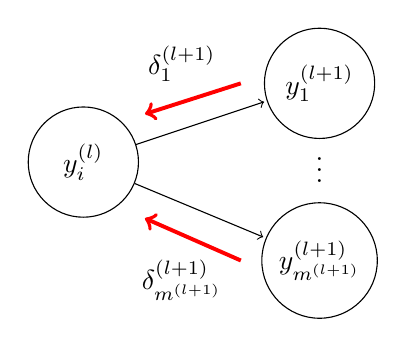
\begin{tikzpicture}[shorten >=1pt]
      		\tikzstyle{unit}=[draw,shape=circle,minimum size =1.4cm]
 
       	\node[unit](i) at (0,1){$y_i^{(l)}$};
        	\node[unit](k1) at (3,2){$y_1^{(l+1)}$};
		\node at (3, 1){$\vdots$};
		\node[unit](km) at (3,-0.25){$y_{m^{(l+1)}}^{(l+1)}$};
		
		\node at (1.25,2.25){$\delta_1^{(l+1)}$};
		\node at (1.25,-0.5){$\delta_{m^{(l+1)}}^{(l+1)}$};
 
        	\draw[->] (i) -- (k1);
		\draw[->] (i) -- (km);
		
		\draw[->,red,line width=0.05cm] (2,-0.25) -- (0.75,0.3);
		\draw[->,red,line width=0.05cm] (2,2) -- (0.75,1.6);
    	\end{tikzpicture}
	\caption[Backpropagation.]{\small{Backpropagation of errors through the network: once evaluated for all output units, the errors $\delta_i^{(L+1)}$ can be propagated backward.}}
	\label{fig:error-backpropagation}
\end{SCfigure}

\newpage


